\documentclass{article}
%\documentclass[journal]{IEEEtran}
%\documentclass{report}
%\documentclass{acta}

\usepackage{graphicx}
\graphicspath{{./media/}}
\begin{document}

\title{Constructing three-dimensional (3D) polycrystalline models of FCC crystal for numerical modeling and simulation with multibody potential}
\author{Rustam Akhunov}

\maketitle

\tableofcontents

\begin{abstract}
The three-dimensional (3D) polycrystalline models of FCC crystal with the log-normal grain size distribution are constructed by constrained Voronoi tessellation. For achieving needed distribution of grain sizes and grain orientation we used Genetic Algorithm (GA) with Least Square (LS). We used molecular-dynamics method in LAMMPS software to obtain the relaxed polycrystal. For the relaxation process and for simulation we used multibody potential.
\end{abstract}


\section{Introduction}

There are known a lot of modern application of polycristalline materials. Polycristallines are used for tritium generation \cite{john99}, automotive, healthcare and non-destructive testing \cite{pardo11}, solar cells \cite{schrop98}, semiconducting elements \cite{harb85} etc. With increasing demand of new properties of new materials increases also need for the modern methods of polycristalline simulation \cite{shen15}. And this work is one more attempt to deal with the simulation of polycryrstallines in molecular dynamics environment such as LAMMPS \cite{plimp95, plimp00}

There are numbers of experiments and theoretical research for the intrinsic structure, effective thermal conductivity, lattice dynamical, optical and thermodynamic properties of polycristalline \cite{shen15}. But still many characteristics have not been researched sufficiently.

We know few methods for generating digital nanostructured materials for use in the simulation: Poisson–Voronoi tessellation (PVT) \cite{wear86}, Monodispersive grain size (MGS) \cite{wang96}, Laguerre–Voronoi tessellation (LVT) \cite{fan04}, Johnson–Mehl (JM) model \cite{okabe00} etc. In this work we used Voronoi tesselation model for the reason of its good solution for the complex sctructural nanocrystals and also convinient interface for the genetic algorithm, that we used during our polycristalline generation. It is also generally accepted that many single-phase fully dense nanocrystals are described by a log-normal grain size distribution. And we took this distribution as a reference for polycristalline generation.

The goal of this work is implementation of general methodology of generation realistic polycrystalline structure. It should correspond grain sizes and orienation distribution, have minimal energy and be relevant to experimental density, lattice constant etc. The methodology also should be fast enough in order to do generation in one or several days on adequate resources. This all we are trying to do using existing results for different polycrystallines.


\section{Overview of existing methods and results}

Before my research I did an overview of existing results in several related papers. One of the most important article for our research was "Constructing three-dimensional (3D) nanocrystalline models of $ Li_4SiO_4 $ for numerical modeling and simulation" \cite{shen15}.

In this paper authors considers problem of generation $ Li_4SiO_4 $ polycrystalline that is  narrowing the result for particular matter. But we rather try to implement more general approach. Of course by making more general method we face much more problem with efficiency and time consuming of the generation method. But even general method can be fitted to the particular element.

The authors use genetic algorithm to reach particular distribution of grain sizes and as we can see they use only mutation operator without crossover. But we in contrary use both mutation and crossover. Moreover we implemented 3 variants of crossover and 3 variants of mutation in order to find optimal operators for our task. We implemented numerous computing experiments and chose optimal combination of operators and other algorithm parameters.

But it is necessary to pay tribute to the good results obtained during implementation of the algorithm. Authors were able to reach very good permormance. In particular the computation time per step was 3.7 s with 6 processors and it is much better compared to the result 3.9 s with 32 processors \cite{suzudo02}.

Even the article mentioned above is a basis for my research I did more deep overview of the topic regarding methods available to generate realistic polycrystalline structure. And one of the intereseting paper dedicated to the problem is "Lattice models of polycrystalline microstructures: A quantitative approach" \cite{rinaldi08}.

Here authors refer to available methods for creating polycrystalline structure. Among several different approaches they mention Voronoi tesselation as a good method for obtaining the polycrystalline structure. It is noticed that this method is very popular and wide spread in fitting to the experimental data and therefore presented in special commercial software such as AMIRA, MIMICS, SURFDRIVER.

Of course Voronoi tesselation method has disadvantages like that it represents only convex polyhedra that is not true for real polycrystals. It is also known that real grains not necessary polyhedra at all. Nonetheless, Voronoi tesselation remains very quick and reliable method of generation structures close to the real polycrystalls. 

In the paper it is also noticed that instead of focusing on precise microstructure much better focus on major statistics like  distribution of grain size and grain orientation. It is actually what I am doing in my work.

However, in the paper the main goal is achieving the mechanically equivalent polycrystalline. Although this approach is good for mechanical properties of material it loses any other aspects of real matter. This is why we cannot apply current results in our research.

Another significant result in realistic generation of polycrystalline structure was achieved in "Mechanical properties of polycrystalline graphene based on a realistic atomistic model" \cite{kotak12}.

Here authors did great work in order to obtain realistic atomic structure of graphene. They implemented algorithm for atomic structure generation based on the growth principle. It means that after random location of grain centers they tried to simulate growth of grains by considering borders of growing grain step by step. They also followed misorientation distribution that have one to one correspondence with orientation distrubution. It is also emphasized the importance of realistic simulation of grain boundaries because of their significant impact on mechanical and electrical properties of material.

The main disadvantages in the work that the result is valid only for graphene and graphene like structures. This limitation I will try to bypass in my work. There is also problem with algorithm used in paper. This approach needs more computing resources and have some difficulties in parallelising. Usually such structure construction need days for obtaining usable results if the system have usual for simulation sizes. The real distribution of grain sizes is absolutely neglected in the paper. It is considered only uniform distribution for the grains that does not follow real structures. But nonetheless, I borowed some ideas for misorientation distribution in my work.

In following "Studying the elastic properties of nanocrystalline copper using a model of randomly packed uniform grains" \cite{guo13} paper I found interesting new approach in studying mechanincal properties of nanoscaled polycrystalline materials. Authors offer concentrate on finding dependency of elastic module on grain boundaries and therefore they make artificial ideal polycrystall where they obtain uniform grain sizes that is not true for realistic structures.

The last very interesting paper to talk about that was considered during literature overview was "Generation of 3D polycrystalline microstructures with a conditioned Laguerre-Voronoi tessellation technique" \cite{falco13}.
Here authors got really singnificant results in obtaining very close to real size distribution polycrystalline structure. In order to do this they used extended Voronoi tessellation method so called Laguerre-Voronoi tessellation. They implemented procedures that allows to associate particles weights with the grains sizes. This method helps to obtain very realistic distribution of grain sizes and use it in the following simulation that they actually did. During simulation using this kind of tessallation they compared simulation results with real experiments with annealed aluminum. Obtained results show high efficiency of this approach and can be used in our work too. Thank to developer of Voro++ library this tessellation is already implemented in the library and we can use Laguerre-Voronoi tesselation as first approximation in our genetic algorithm. It can significantly improve time of calculation.

Now from the papers about theoretical statements we move to the practical results that currently exist and can help to generate polycrystalline structure.

Firstly, I would like to mention very useful modern software so called nanoSculpt \cite{prak16}. It allows to construct atomic structure inside any shape and forms. It also support constructing of Voronoi tessellation for polycrystalls in any shape. It was written using C language and easy extensible enough. But unfortunatelly, currently this package does not support following particular distribution of grain size and orientation during costruction of structure. 

Another interesting tool is AtomEye \cite{juli03} developed by MIT staffs. It is very comprehensive and powerfull tool for dealing with atomic structure. One of the most interesting util for me in this package is so called voronoirize tool. It can be used for building polycrystalline structures. The software is written in C language. But again problem it does not follow user defined distributions of sizes and orientations. 

And the last tool that I would like to mention is Atomsk \cite{hirel15}. According to the website title of the utils it is the Swiss-army knife of atomic simulations. It supports many and many methods for atomic simulation. You can obtain numereous output format for any simulation programs you need. But I faced the same problem as in mentioned above tools. To generate polycrystalline structure with particular distributions you need to define orientation and size for each grain by hand. It is not convinient in particular with big sized simulation boxes. Moreover this util is written in Fortran language that is not very convinient tool for wide support and extension. Particularly in industry field.

As you can see there are many researchs and tool dedicated to the problem of generating of polycrystalline structures. But there are several problems that you can face while using them. Firstly they do not support generation based on user defined distribution that makes these tools very hard to use in realistic conditions. Secondly, tools and methods which support realistic structures work on very slow algorithm that needs days for obtaining trustful results. Thirdly, sometimes tools are written in "not good" languages and are hard to maintain.

These all reasons inspired me to create useful tool for generating realistic polycrystalline structure written in C++ language and backed by LAMMPS simulation software.

\section{Building the Voronoi tessellation}

As it was mentioned above we use Voronoi tessellation for building our polycrystalline structure. But for obtaining real stucture we have to fit some properties of natural crystalls during generation of tessellation. In our work we are especially interested in fitting tessellation to the two crucial distributions: grain size distribution and grain orientation distribution. All generation done in periodic condition of the boundary.

\subsection{Building the Voronoi tessellation fitting the given grain size distribution}

In our generation process we tested several distributions for grain size but only one of them was chosen as a discribution for real polycsystall, it is lognormal distribution \cite{shen15, liu14}.

As far as we have a set of 3D points in the space as a individual we are considering all operators acting on these points because we do not have any other objects to deal with.
So, crossover operator just exchange points between two individuals according to the some rule defined in the implementation. And mutation operator just shifts the given points of individual according to the defined probability.

For fitting grain size distribution we used genetic algorithm. In order to find best conditions of algorithm convergence we implemented several variants for crossover and mutation operator. Especially for crossover we have one-point, two-point and uniform crossover. First and second variants just straightforward classcial implementation of the operator. While uniform crossover is kind of nonstandard variant where point-to-point exchange rule follow random distribution. In other words, we take one point from first individual and randomly exchange with random point from the second individual. While in one- and two-point crossover we exchange points according to the virtual distance between  them. Particularly, we exchange point if they are close to each other. You can see this mapping on Figure \ref{mappingindividuals}.

Here on the figure blue colored dots are points of first individual and red ones are of the second individual. We are making pairs of points from first and second individual according to the shortest distance between them. Green lines show which points we chose for pairing. As you can see in each case pairs are made between closest points.
 
\begin{figure}
    \centering
    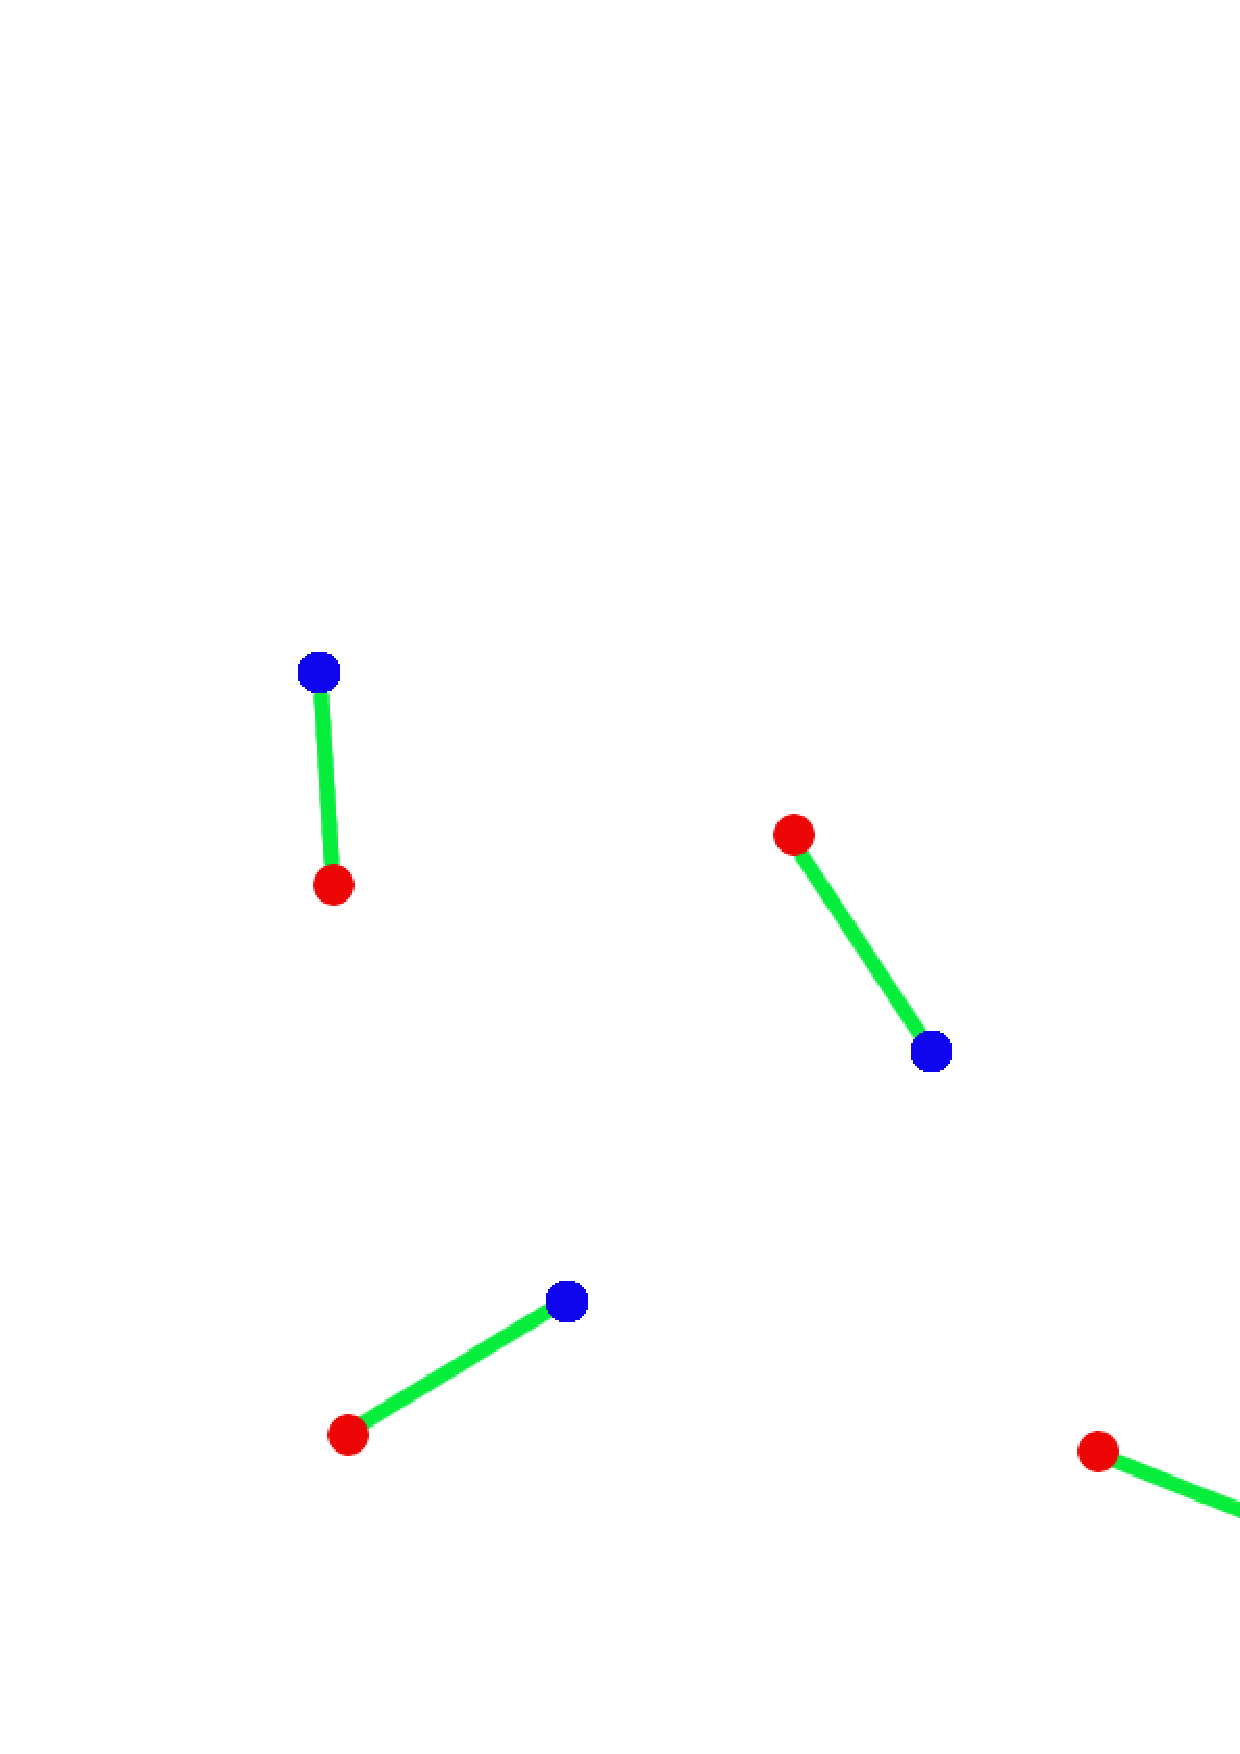
\includegraphics[width=3.0in]{individuals_map}
    \caption{Mapping of two individuals' points}
    \label{mappingindividuals}
\end{figure}

For the mutation operator we implemented variant with different distribution for point shifting value. Especially we implemented and tested two kind of distribution: uniform and normal. The maximum aplitude for the shifting is adopting to the system under consideration. We compute average volume for the one particle by dividing the whole simulation box by the amount of particles. After we take to cube root of this volume and obtain the adopted shifting maximum amplitute for the mutation operator.

Another variant for the mutation operator it is just reinitialization of the given point. 

If we generalize the whole algorithm we implemented we can highlight 4 parameters that impact on the convergence and convergence speed of the genetic algorithm. They are crossover operator type, mutation distribution, mutation probability and population size.

By changing and variating the set of these parameters we obtain particular configuration of the algorithm. Our goal is to find the optimal configuation when the algorithm will converge and will do it quickly enough.

In order to obtain the optimal configuration we chose some dicrete values for population size and mutation probability and assemble all possible configurations from these values. For mutation probability we considered values 0.8, 0.2, 0.05, 0.01. For population size we considered 10, 40, 100. For operators variants are already discrete. Namely, for crossover operator: one-point, two-point and uniform and for mutation: uniform, normal, reinitialization. All these configurations are accepted by the bash script as a parameter that makes testing of all possible configurations easy enough.

For each particular configuration we run 48 instances due to our idea to find the mean value and standard deviation for each considered point.

For aggregation data from each configuration runs and finding mean value and standard deviation we used python pandas module.

The results for best, worst and average penalty for different configuration are presented on Figures \ref{crossovercomp1}, \ref{crossovercomp2}, \ref{crossovercomp3}, \ref{mutationprobcomp1}, \ref{mutationprobcomp2}, \ref{mutationprobcomp3}.


\begin{figure}
    \centering
    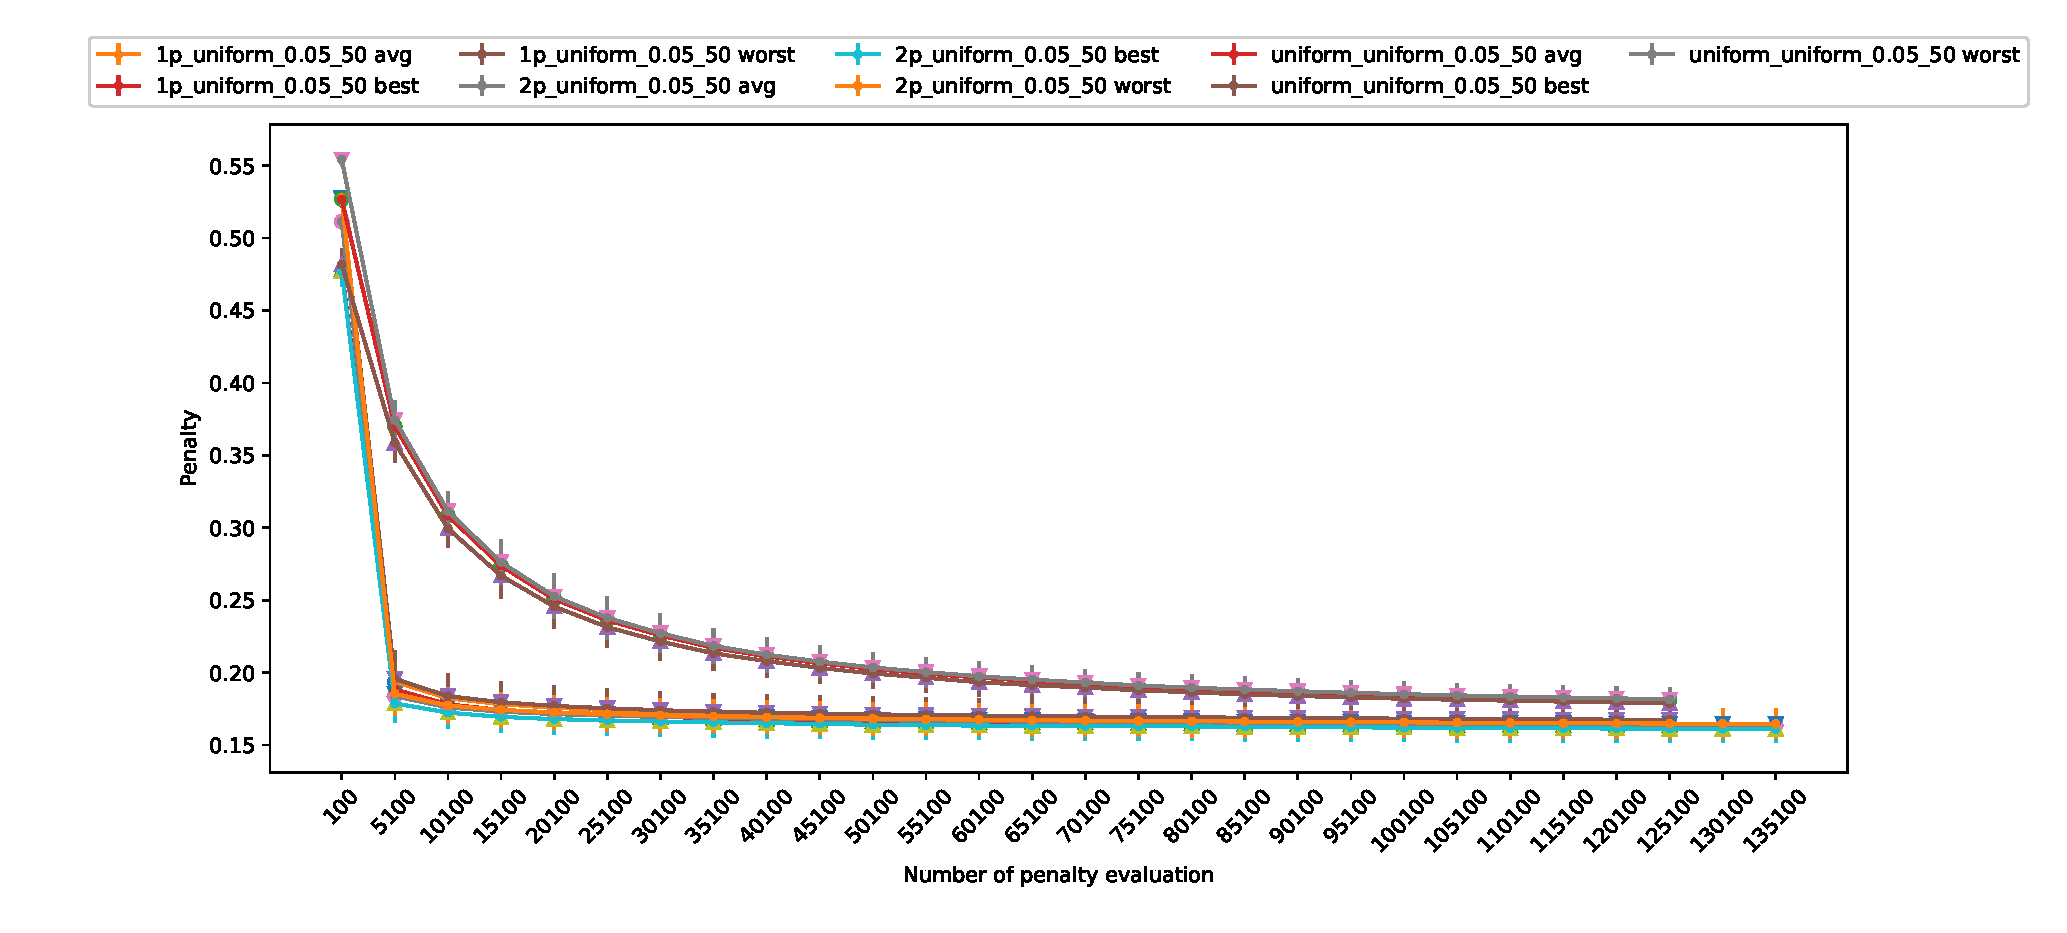
\includegraphics[width=5.0in]{crossover_comparison_md_uniform}
    \caption{Comparison of crossover operators while mutation distribution is uniform}
    \label{crossovercomp1}
\end{figure}

\begin{figure}
    \centering
    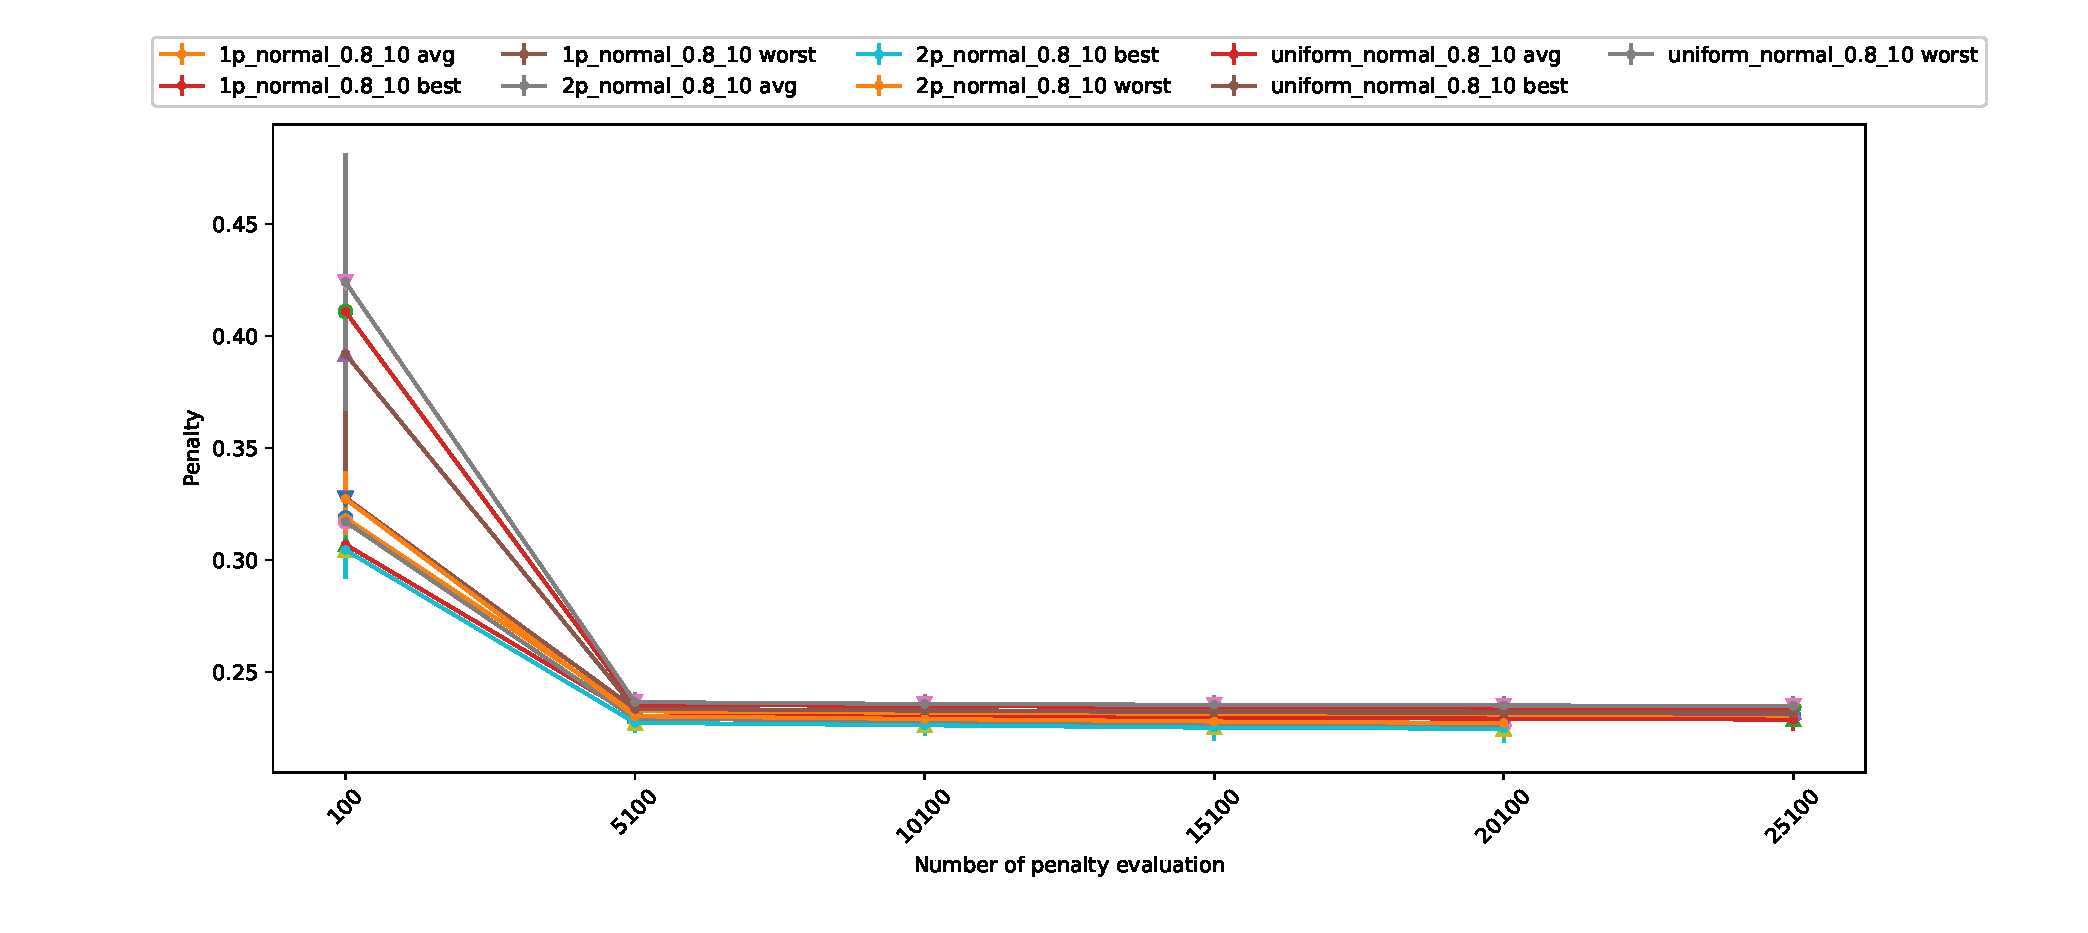
\includegraphics[width=5.0in]{crossover_comparison_md_normal}
    \caption{Comparison of crossover operators while mutation distribution is normal}
    \label{crossovercomp2}
\end{figure}

\begin{figure}
    \centering
    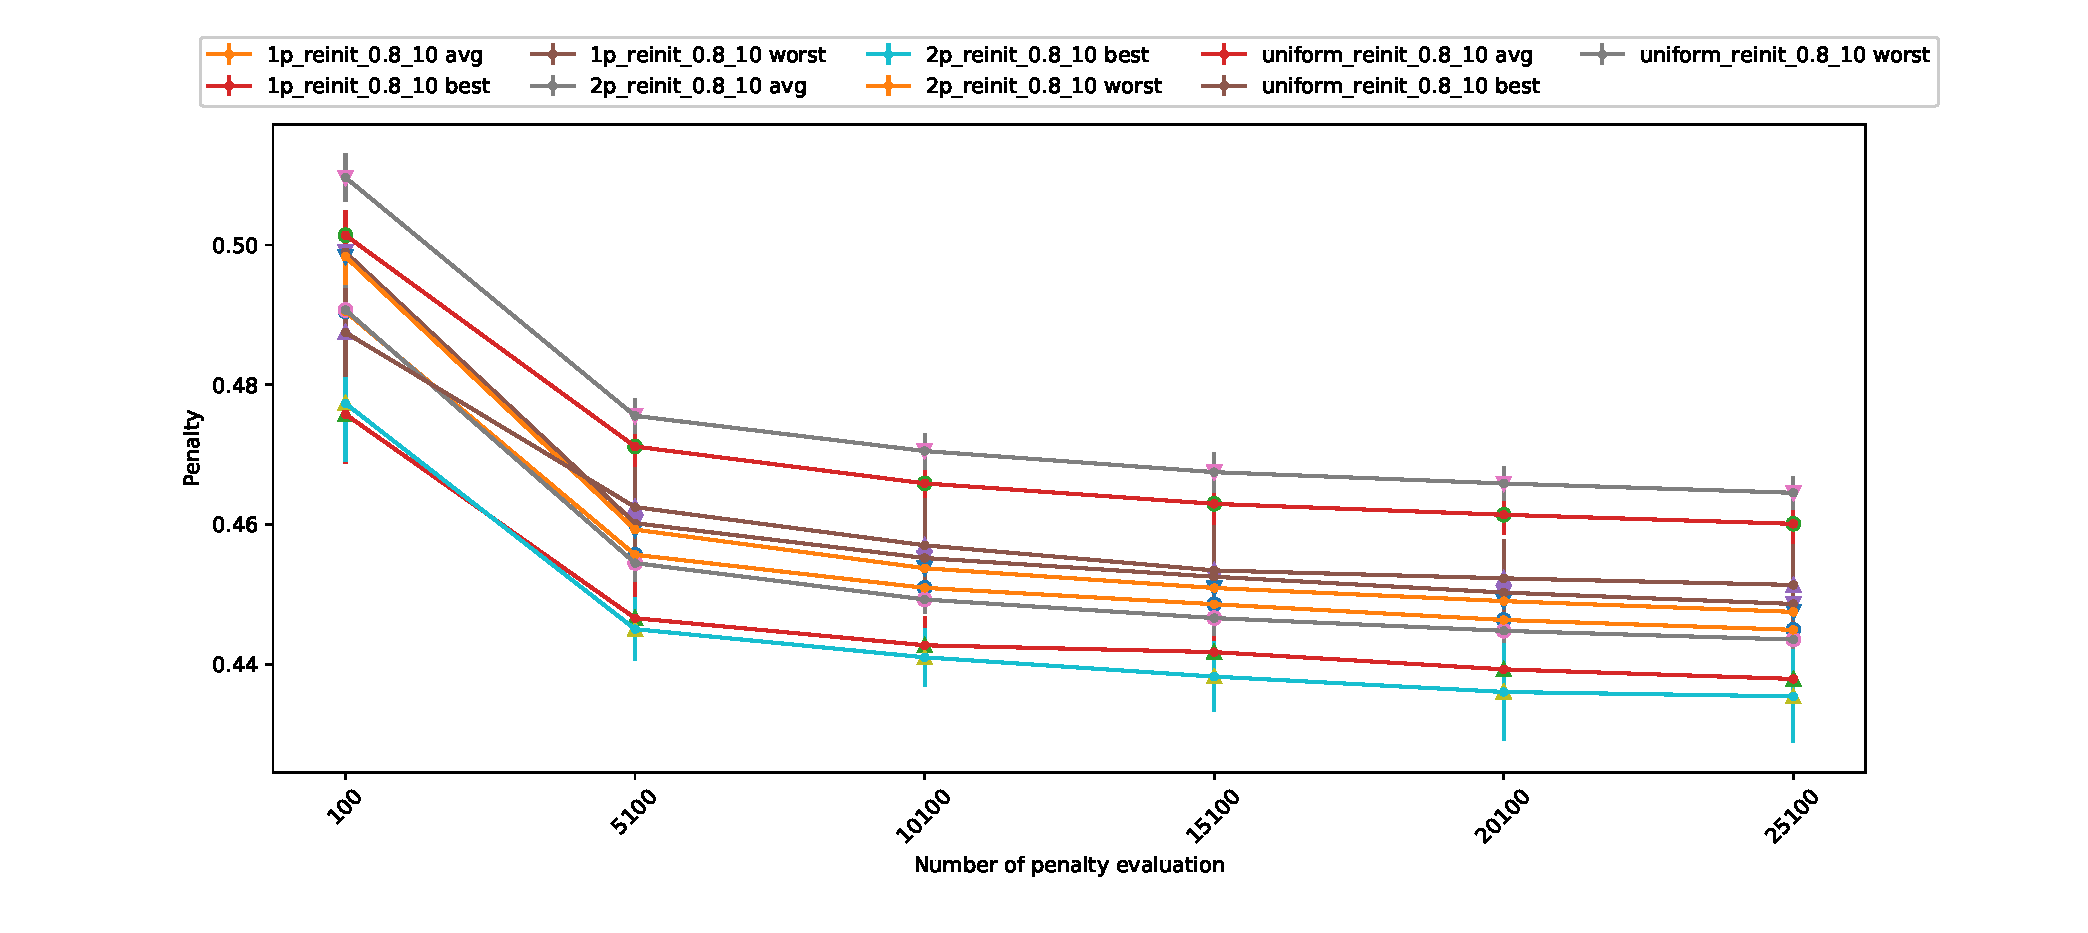
\includegraphics[width=5.0in]{crossover_comparison_md_reinit}
    \caption{Comparison of crossover operators while mutation is just reinitialization}
    \label{crossovercomp3}
\end{figure}

\begin{figure}
    \centering
    \includegraphics[width=5.0in]{mutation_probability_comparison_population_10}
    \caption{Comparison of mutation probability while population size is 10 individuals}
    \label{mutationprobcomp1}
\end{figure}

\begin{figure}
    \centering
    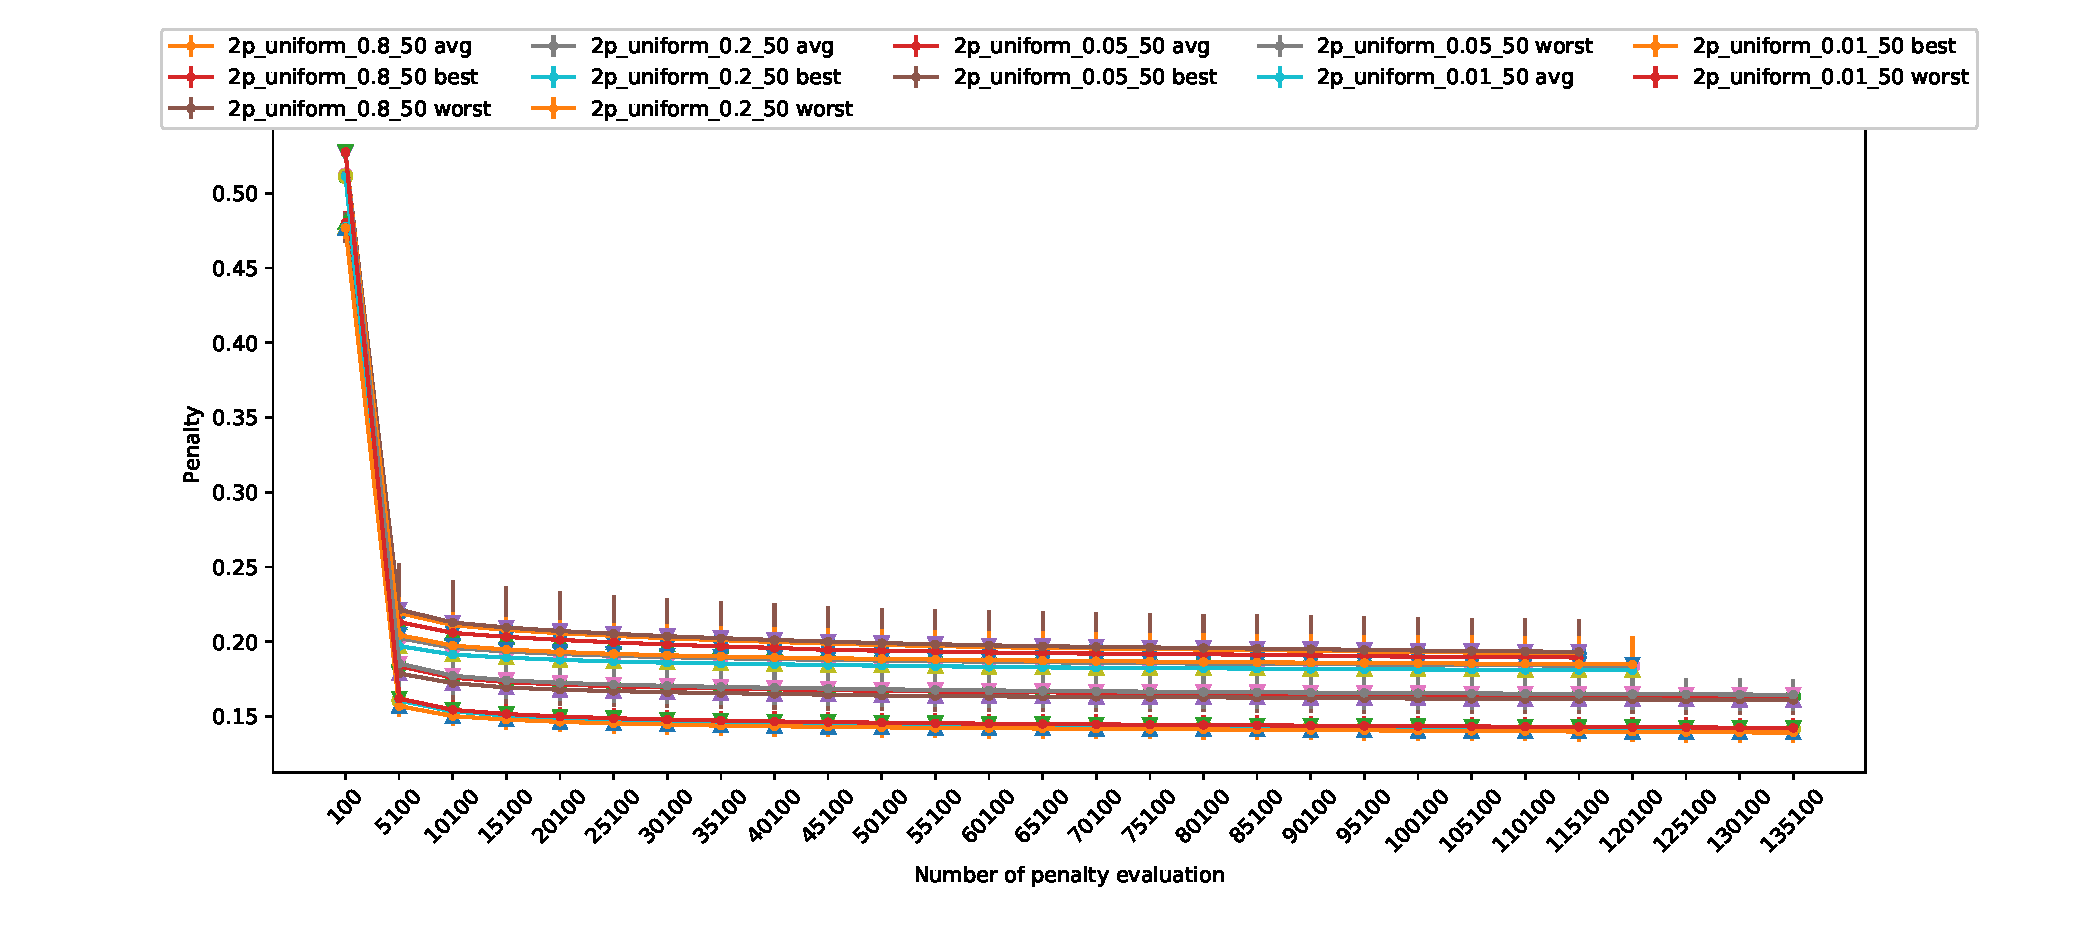
\includegraphics[width=5.0in]{mutation_probability_comparison_population_50}
    \caption{Comparison of mutation probability while population size is 50 individuals}
    \label{mutationprobcomp2}
\end{figure}

\begin{figure}
    \centering
    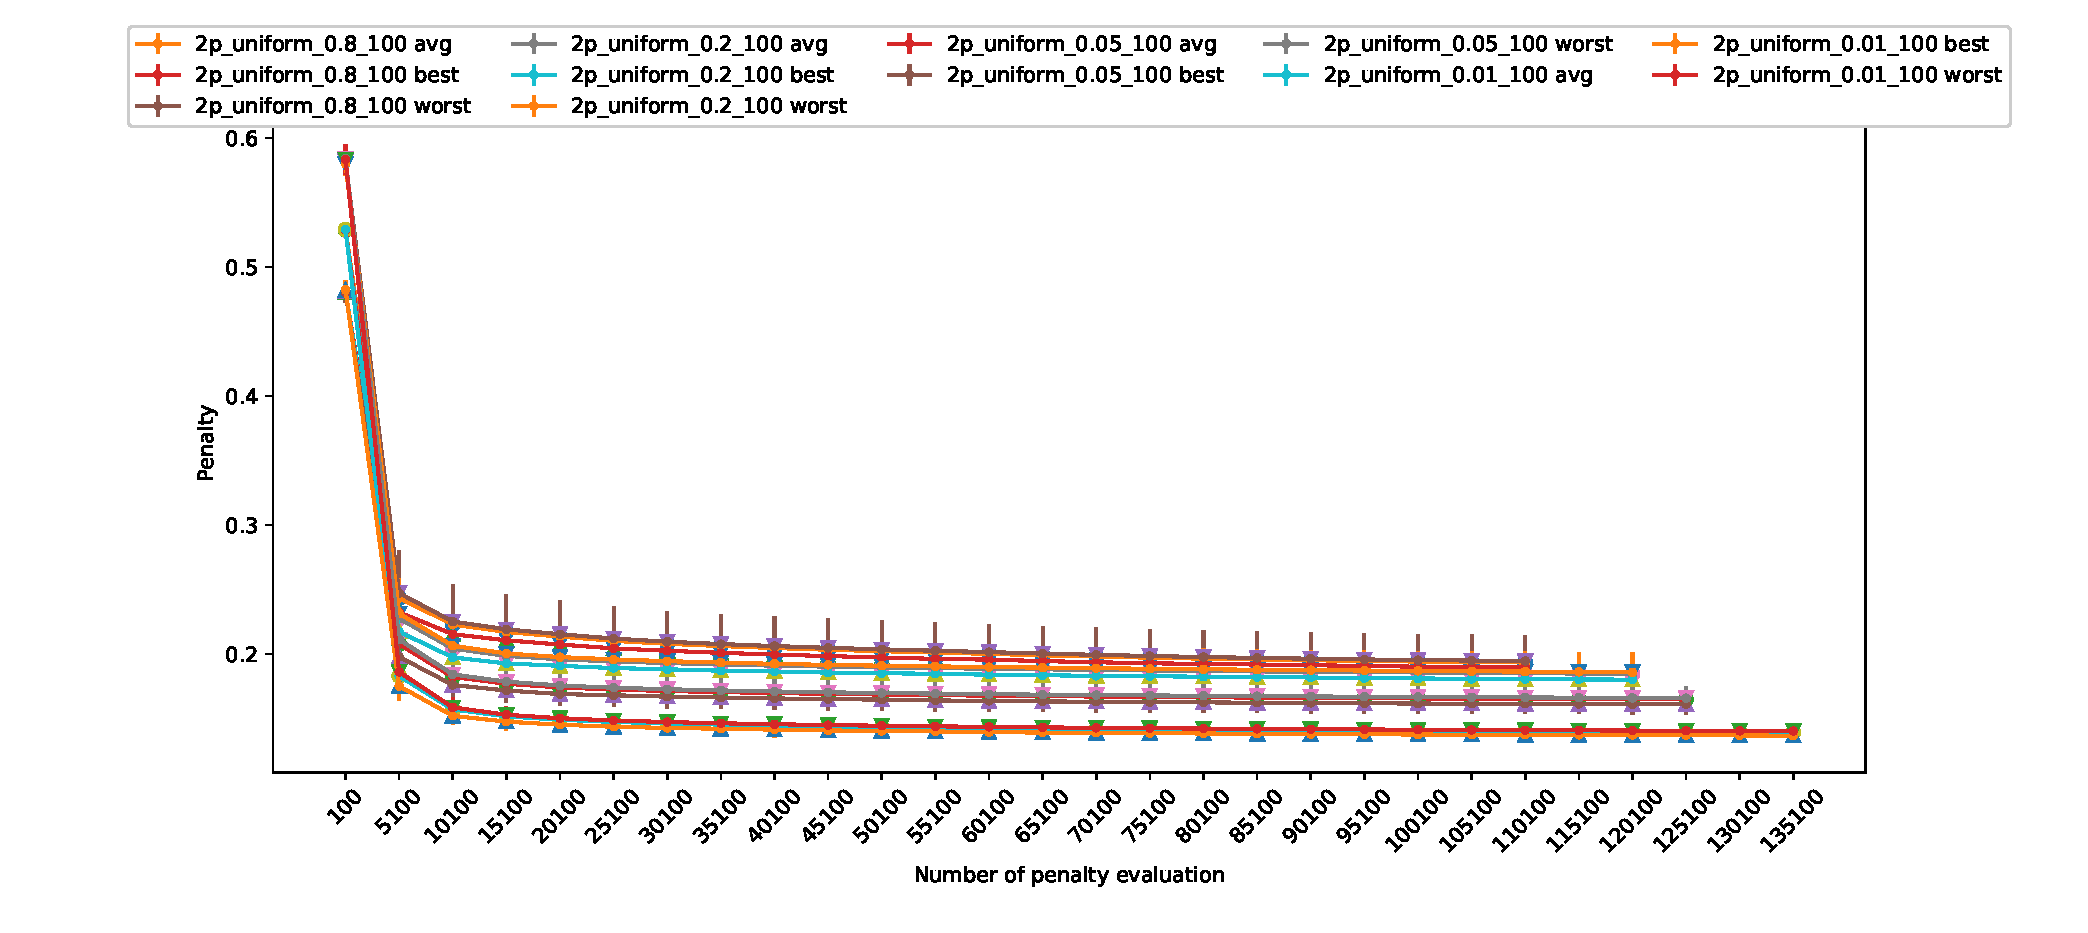
\includegraphics[width=5.0in]{mutation_probability_comparison_population_100}
    \caption{Comparison of mutation probability while population size is 100 individuals}
    \label{mutationprobcomp3}
\end{figure}

\begin{figure}
    \centering
    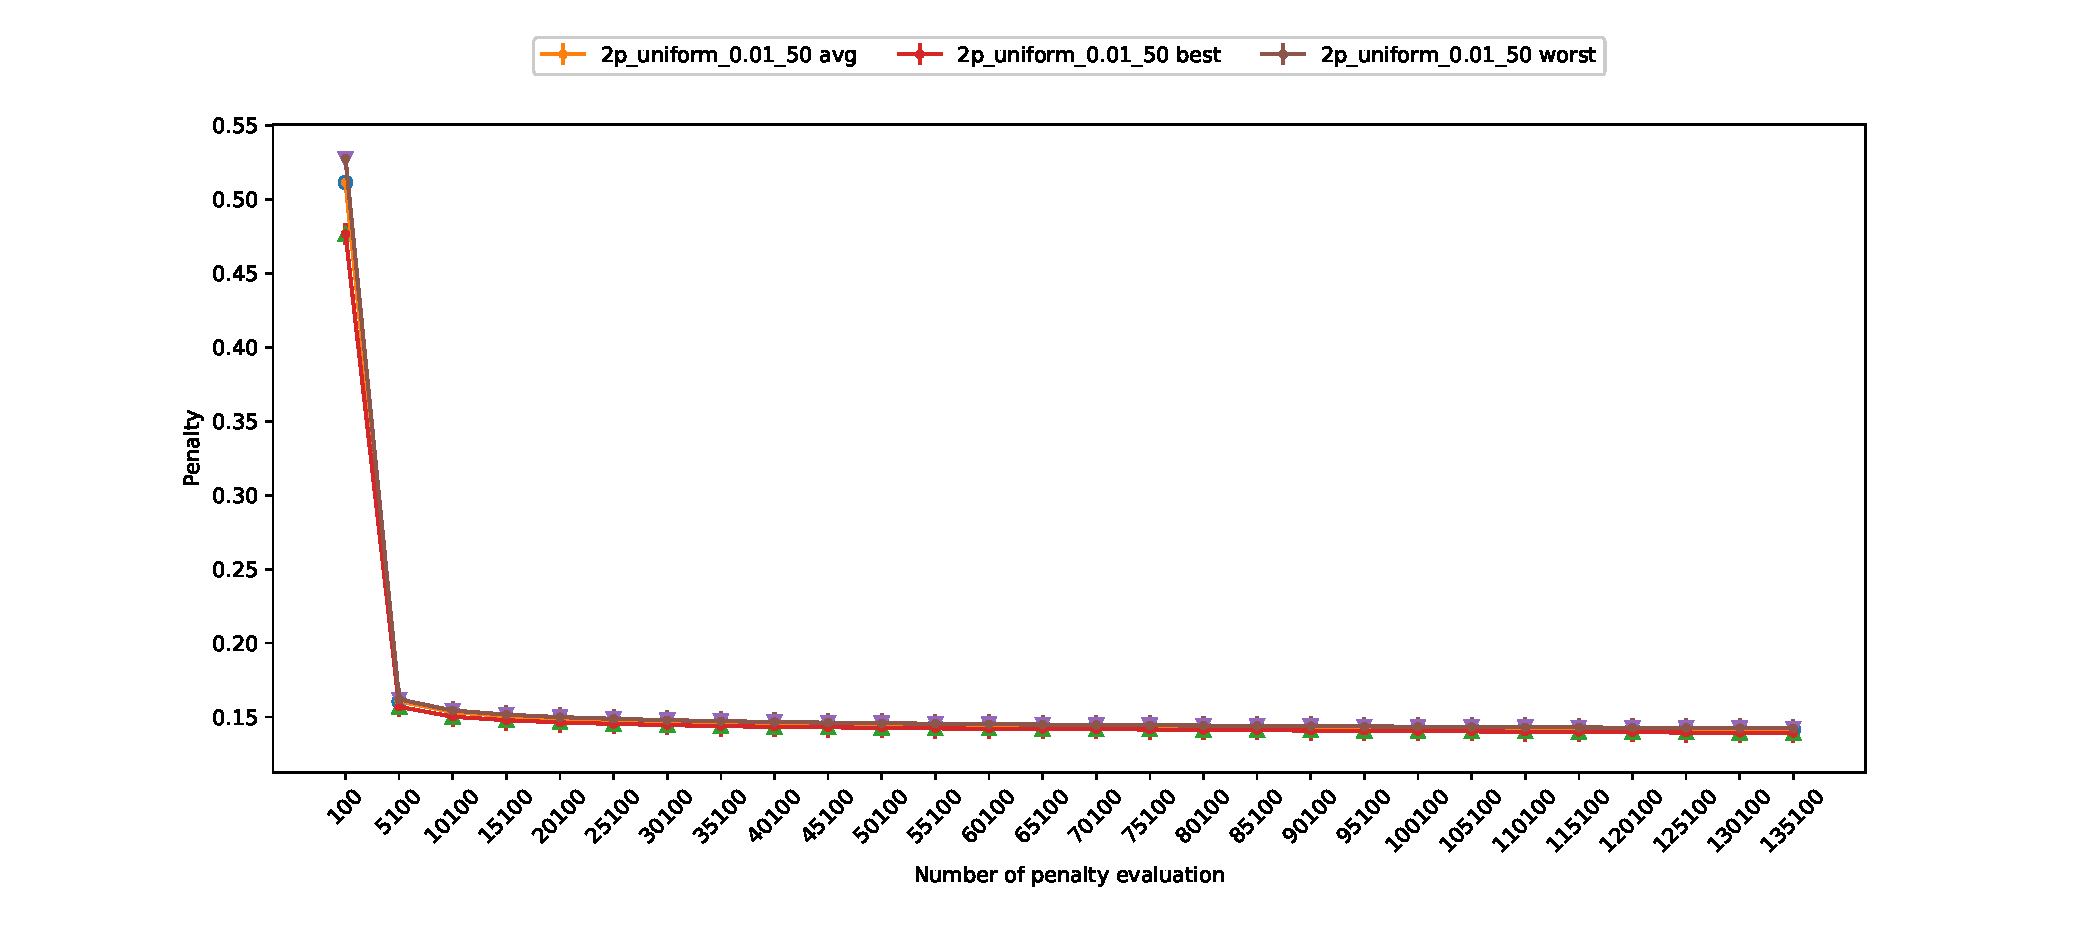
\includegraphics[width=5.0in]{best_configuration}
    \caption{The best configuration: 50 individuals, 0.01 mutation probability, two point crossover, uniform distribution for mutation}
    \label{bestconfiguration}
\end{figure}

\begin{figure}
    \centering
    \includegraphics[width=5.0in]{first_last_comparison}
    \caption{The result of genetic algorithm work after 3000 steps}
    \label{firstlastcomp}
\end{figure}

On these figures there are presented 3 lines: the best individual's penalty, the worst individual's penalty and the average penalty for the number of evaluating of penalty function.

I permormed optimal configuration finding strategy in following manner. As we have 4 parameters for each configuration I divided this set to two subsets with two paremeters in each. Then in each subset I run calculations with different parameters from the set while parameters outside set were fixed. E.g. in \ref{crossovercomp1} we comparing crossover operators while mutation is uniform and population size and mutation probability are fixed. Similarly for \ref{crossovercomp1} with except of mutation operator. Here this operator has normal distribution, but all other parameters have the same set of values. 

On the labeles above the graphs you can see titles of lines presented on the charts. Titles encode the configuration of the current line. For example "2p\textunderscore uniform\textunderscore 0.1\textunderscore 20 worst" means we have two-point crossover operator, uniform distribution for mutation, 0.1 mutation probability and 20 population size. Word "worst" means that all values presented for the worst individual in the current population. Besides "worst" we also have "best" and "avg". "Best" means values for the best individual and "avg" means average values for the generation.

After permorming a lot of calculations we came to conclusion that "2p\textunderscore uniform\textunderscore 0.01\textunderscore 50" is the best configuration in terms of convergence.

\subsection{Building the Voronoi tessellation fitting the given grain orientation distribution}

For reaching selected grain orientation distribution we also used genetic algorithm. But it is supposed to use this optimization only after reaching grain size distribution because in case of grain orientation we do not change tessellation but rather we change only orientation of the grains.

Each orientation is represented by Euler angles. Although we have orientation for each grain we are interested in relative orientation between grains. We introduce this orientation as a difference between orientations of two selected grains. It can be imagined as angles needed to rotate first orientation in order to obtain the second orientation and vise versa.

In particular we use the same crossover operators for choose which points we have to exchange but instead of exchanging points theirselves we exchange their orientations and leave points positions intact. Therefore we need only one individual of tessellation and many configuration of orientation.

For mutation operator we change slightly the Euler angles of the grain. We consider only one octant with angles from 0 to pi/2 because we are dealing only with cubic lattice in this work. Latter on outside of this work we will work with more complex lattices.

We can think about two algorithms for grain sizes and grain orientation as a similar problems with the similar properties. For example, when we change position of one point in grain size algorithm we change sizes of current cell and all neighboring cells. The same for grain orientation algorithm. When we change orientation for one cell we change all relative orientation around particular grain.

For grain orientation algorithm we also have the set of possible parameters that influence on the convergence. They are the same as for grain size algorithm. We also have to find optimal configuration for the algorithm and this is why we performed the same procedure of calling script that variates all possible configuration. After running all configuration several times (48 times) we in the same way calculate mean value and standard deviation. Here are results of worst, best and tree medium configurations:

\[figures representing grain orientation algorithm results\]

\section{Filling tessellation with particles (atoms)}

After obtaining fitted Voronoi tessellation we have to fill it with the atoms. The filling should correspond to the reached grain orientation distribution. In order to do this we generate lattice with given lattice constant arround the grain point with size exceeding grain size twice to cover all possible artifacts during rotation. After that we rotate generated set of atoms by the euler angles that we got during grain orientation optimization. Now we cut all redundant atoms that lie outside of the considered grain and so we have filled grain of the polycrystalline.

The only trick that we need during this generation is following the periodic condition of the system. This is why if we have grain touching the boundary of the simulation box we need to transfer atoms to the corresponding part of grain lying in the opposite side of the box.  

\section{Relaxation of atomic structure}

The relaxation process in this work backed by minimization of whole energy by shifting the center of lattice generation for each grain and by removing some atoms on grains borders. Calculating of whole energy performed by LAMMPS module. For calculating energy we use many body potential \[the name and formula for potential\].

The process of generation center shifting is implemented again by using genetic algorithm. We generate randomly generation and for each individual calculate total energy. Crossover and mutation are implemented in similar way as it was for grain size genetic algorithm with the exception that we deal with center of generation and leave untouched the tessellation.

After achieving optimal low energy we walk through border of each grain and try to remove redundunt atoms again in order to lower total energy.

If we found that structure is stable we run simulation in LAMMPS with chosen potential to finish the process of relaxation and hence by the end we obtain realistic polycrystalline structure.

\section{Results and discussion}

- describe how we did genetic algo for different configurations for sizes and orientations and show the common graph for all configurations
- discuss about why is it so. why it works with these parameters
- describe more detailed and with graphs the filling processs and discuss the results
- descibe in detail relaxation process and show progress of total energy reduction

\section{Methods}

- show block scheme of genetic algo for sizes and orientation
- show block scheme for filling
- show block scheme for relaxation
 
\section{Additional Information}

???

\section{Conclusion}



\begin{thebibliography}{9}

\bibitem{john99}
  Johnson C. E. J.
  \textit{Tritium behavior in lithium ceramics}
  Nucl. Mater
  1999

\bibitem{pardo11}
  Pardo, Lorena, Ricote, Jesús (Eds.)
  \textit{Multifunctional Polycrystalline Ferroelectric Materials}
  Springer
  2011

\bibitem{schrop98}
  Schropp, Ruud E. I. Zeman, Miro
  \textit{Amorphous and microcrystalline silicon solar cells : modeling, materials, and device technology}
  Boston (Mass.) : Kluwer academic
  1998.

\bibitem{harb85}
   Harbeke, G. (Ed.)
  \textit{Polycrystalline Semiconductors}
  Springer-Verlag Berlin Heidelberg
  1985

\bibitem{plimp95}
   S. Plimpton 
  \textit{Fast Parallel Algorithms for Short-Range Molecular Dynamics}
  J Comp Phys, 117, 1-19
  1995

\bibitem{plimp00}
   S. Plimpton 
  \textit{LAMMPS WWW Site}
  http://lammps.sandia.gov

\bibitem{shen15}
  Shen, Y. et al. 
  \textit{Constructing three-dimensional (3D) nanocrystalline models of Li4SiO4 for numerical modeling and simulation.}
  Sci. Rep. 5, 10698; doi: 10.1038/srep10698 
  2015

\bibitem{suzudo02}
  Suzudo T.  Kaburaki H. 
  \textit{An evolutional approach to the numerical construction of polycrystalline structures using the Voronoi tessellation}
  Phys. Lett. A 373, 4484–4488 (2009).

\bibitem{wang96}
  Wang J. et al. 
  \textit{Computer simulation of the structure and thermo-elastic properties of a model nanocrystalline material}
  Philos. Mag. A. 73, 517–555 
  1996

\bibitem{rinaldi08}
  Antonio Rinaldi, Dusan Krajcinovic, Pedro Peralta, Ying-Cheng Lai
  \textit{Lattice models of polycrystalline microstructures: A quantitative approach}
  Mechanics of Materials 40 (2008) 17–36

\bibitem{kotak12}
  Jani Kotakoski and Jannik C. Meyer
  \textit{Mechanical properties of polycrystalline graphene based on a realistic atomistic model}
  Phys. Rev. B 85, 195447 – 24 May 2012

\bibitem{guo13}
  Guo-Jie J. Gao  Yun-Jiang Wang Shigenobu Ogata
  \textit{Studying the elastic properties of nanocrystalline copper using a model of randomly packed uniform grains}
 Computational Materials Science
Volume 79, November 2013, Pages 56-62

\bibitem{prak16}
  A.Prakash M.Hummel S.Schmauder E.Bitzeka
  \textit{Nanosculpt: A methodology for generating complex realistic configurations for atomistic simulations}
 MethodsX
Volume 3, 2016, Pages 219-230

\bibitem{juli03}
  Ju Li
  \textit{AtomEye: an efficient atomistic configuration viewer}
 Modelling Simul. Mater. Sci. Eng. 11 (2003) 173–177

\bibitem{hirel15}
  Pierre Hirel
  \textit{Atomsk: A tool for manipulating and converting atomic data files}
 Computer Physics Communications
Volume 197, December 2015, Pages 212-219

\bibitem{falco15}
  SimoneFalco JiaweiJian Francesco De Cola Nik Petrinic
  \textit{Generation of 3D polycrystalline microstructures with a conditioned Laguerre-Voronoi tessellation technique}
 Computational Materials Science
Volume 136, August 2017, Pages 20-28


\bibitem{wear86}
  Weaire D. et al. 
  \textit{On the distribution of cell areas in a Voronoi network}
  Philos. Mag. B 53, 101–105 
  1986

\bibitem{fan04}
  Fan Z. G. et al. 
  \textit{Simulation of polycrystalline structure with Voronoi diagram in Laguerre geometry    based on random closed packing of spheres} 
  Comput. Mater. Sci. 29, 301–308 
  2004

\bibitem{okabe00}
Okabe A. et al. 
\textit{Spatial Tessellations-Concepts and Applications of Voronoi Diagrams}
Wiley, New York, 
2000

\bibitem{sivan98}
  S. N. Sivanandam , S. N. Deepa
  \textit{Introduction to Genetic Algorithms},
  Springer Publishing Company, Incorporated
  2007

\bibitem{melan98}
  Melanie Mitchell
  \textit{An Introduction to Genetic Algorithms}
  MIT Press, Cambridge, MA
 1998

\bibitem{suwas14}
  S. Suwas and R. K. Ray
  \textit{Crystallographic Texture of Materials}
  Springer-Verlag London 
  2014

\bibitem{liu14}
  Xuan Liu, Andrew P. Warren,
  \textit{Comparison of crystal orientation mapping-based and image-based measurement of grain size and grain size distribution in a thin aluminum film}
  Acta Materialia 79, 138–145
  2014

\end{thebibliography}


\section{Acknowlegments}

\end{document}
